\chapter{Background}
\label{ch:background}

% Choose your own headings.

\section{Background}

In my researches the non-profit websites that excel tend to have a few key characteristics: clear mission statements, easy navigation, compelling content, and strong calls to action that encourage visitor engagement, such as donations or volunteering.

This review examines related projects, techniques, and methods relevant to this initiative, highlighting the effectiveness and gaps that our project intends to fill.

The \textit{Praia Limpa Santa Marta} project aims to create a non-profit website dedicated to conserving nature and promoting the 'leave no trace' principle in Farol de Santa Marta, Brazil. This review examines related projects, techniques, and methods relevant to this initiative, highlighting the effectiveness and gaps that our project intends to fill.

\section{Literature Review}

The literature review section examines existing research and projects that relate to the objectives of the \textit{Praia Limpa Santa Marta} project, highlighting both their successes and shortcomings to establish a foundation for the proposed initiative.

\subsection{Environmental Conservation and Non-Profit Web Platforms}
Non-profit organizations have increasingly turned to digital platforms to engage the public in environmental conservation efforts. Websites like Charity: Water\cite{charitywater} and World Wildlife Fund\cite{wwf} have set benchmarks in using compelling narratives and visual storytelling to mobilize support and generate donations. Charity: Water, for example, excels in using high-quality imagery and engaging content to communicate its mission of providing clean water in developing countries, as shown in Figure \ref{fig:charity_water}. Similarly, the WWF’s use of powerful imagery and concise messaging effectively advocates for nature conservation, as seen in Figure \ref{fig:WWF}. These examples underscore the importance of clear mission statements, easy navigation, and strong calls to action in non-profit websites.

However, while these platforms have been successful in raising awareness and funds on a global scale, they often lack localized approaches that cater to the specific needs of small communities. For instance, the global reach of the WWF, while impactful, does not necessarily translate into targeted, community-specific actions that are crucial for the success of localized initiatives like \textit{Praia Limpa Santa Marta.} This highlights the need for a platform that combines the strengths of these successful models with a focus on local community engagement and tailored environmental strategies.

\begin{figure}[h]
    \centering
    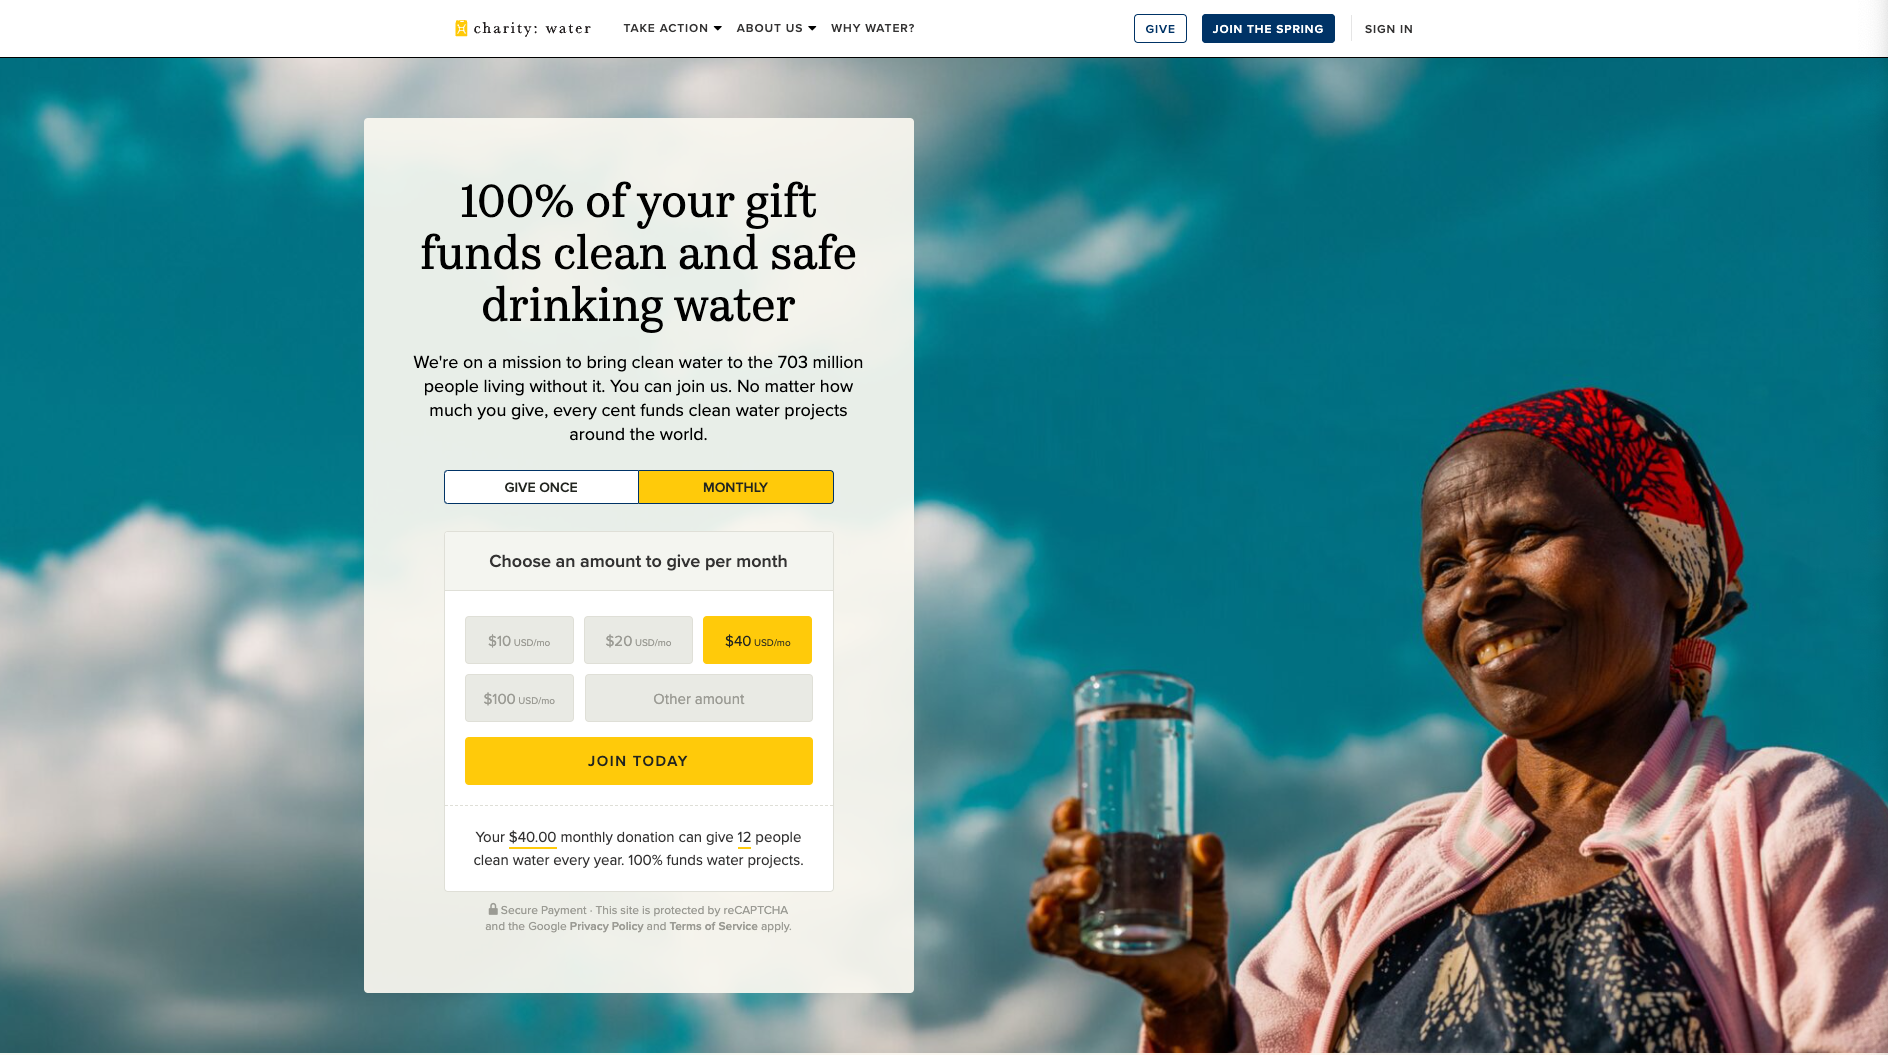
\includegraphics[width=1\linewidth]{images/charity_water.png}
    \caption{Charity: Water}
    \label{fig:charity_water}
\end{figure}

\begin{figure}[h]
    \centering
    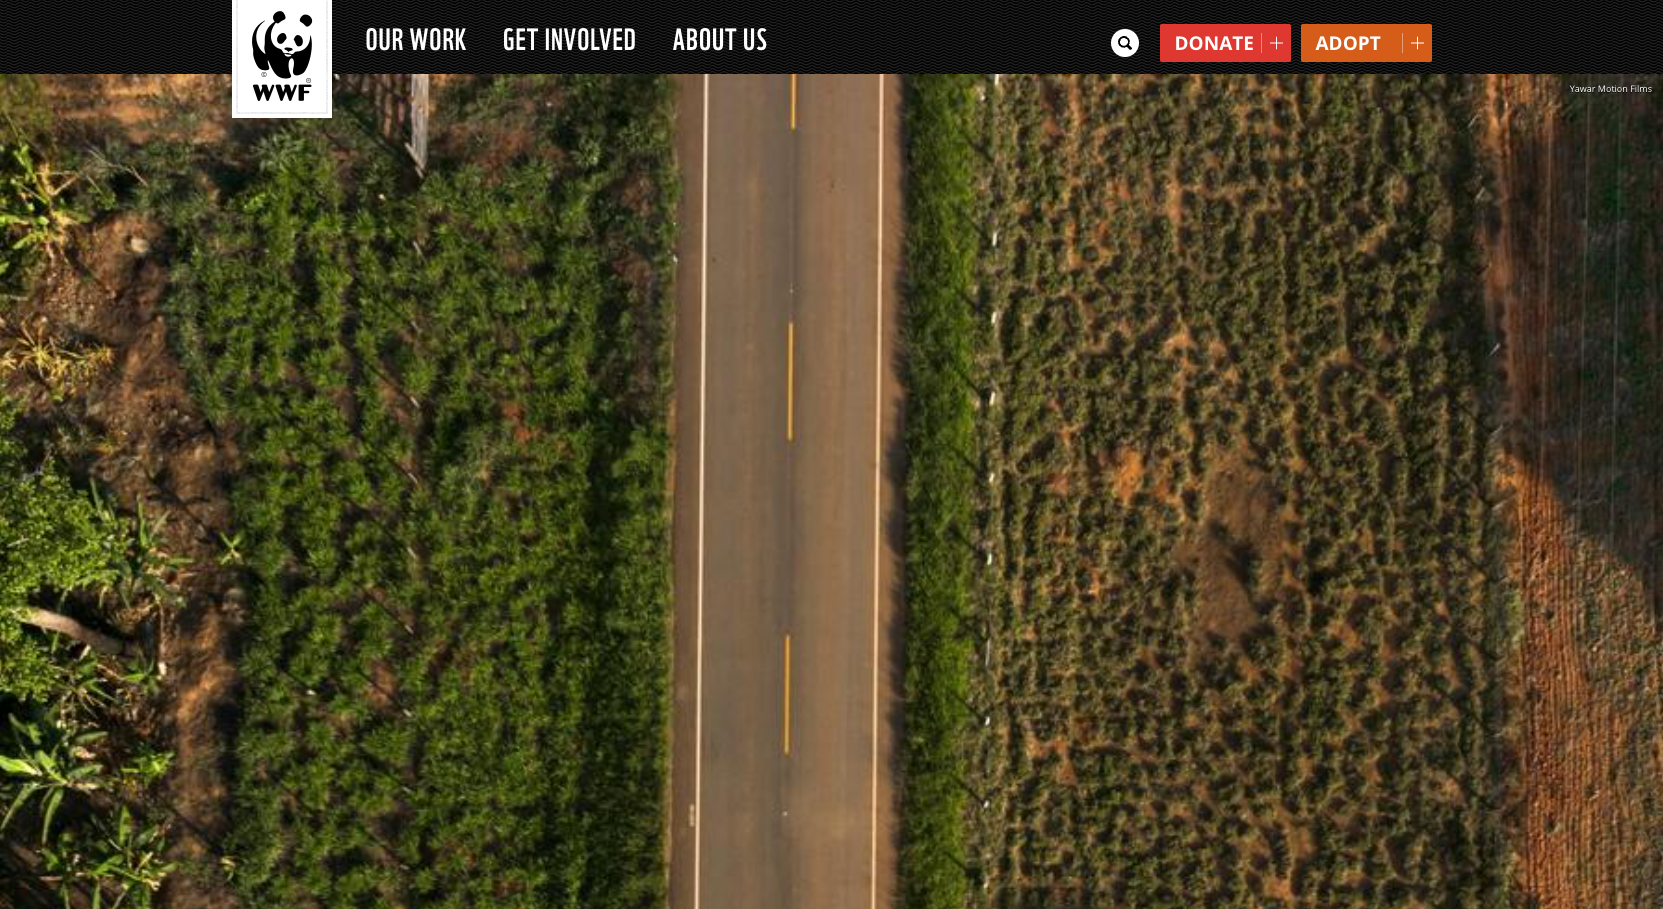
\includegraphics[width=1\linewidth]{images/WWF.png}
    \caption{World Wildlife Fund (WWF)}
    \label{fig:WWF}
\end{figure}



\subsection{Community-Based Conservation Efforts}

The importance of community engagement in conservation efforts cannot be overstated. Studies like those by Western and Wright\cite{western1994} in \textit{Natural Connections: Perspectives in Community-Based Conservation} emphasize the critical role that local communities play in the success of conservation initiatives. The authors argue that sustainable conservation is only possible when the community is actively involved in decision-making and implementation processes. This principle is central to the \textit{Praia Limpa Santa Marta} project, which aims to empower the local community by providing them with the tools and resources necessary to take ownership of their environmental challenges.

Despite the proven importance of community involvement, many conservation projects fail to engage local populations effectively. Initiatives such as the \textit{Beach Clean Brasil} campaign, while successful in mobilizing volunteers, often lack the educational components necessary for fostering long-term environmental stewardship. This gap points to the need for integrating educational programs into the \textit{Praia Limpa Santa Marta} platform to ensure that community members not only participate in clean-up activities but also develop a deeper understanding of the importance of conservation.

\subsection{Tourism and Environmental Impact in Farol de Santa Marta}

Tourism has a profound impact on the social and environmental dynamics of coastal communities like Farol de Santa Marta. The ethnographic research conducted by Santos and Arantes\cite{dosSantos2010} provides valuable insights into how tourism has transformed this traditional fishing village into a popular tourist destination. The influx of tourists has brought economic benefits but also significant environmental challenges, including increased waste and pollution.

The study highlights the need for sustainable tourism practices that balance economic benefits with environmental preservation. This is where the \textit{Praia Limpa Santa Marta} project can make a significant contribution by promoting responsible tourism through its digital platform. By educating tourists about the 'leave no trace' principle and providing them with opportunities to participate in local conservation efforts, the project aims to mitigate the negative environmental impact of tourism in the region.

\subsection{Technological Solutions for Environmental Conservation}

The use of technology in environmental conservation has opened new avenues for engagement and impact. Web-based platforms offer a scalable solution for mobilizing communities, educating the public, and facilitating conservation activities. The choice of Django for the development of the \textit{Praia Limpa Santa Marta} platform reflects a strategic decision to leverage robust and flexible technologies that can handle the complexities of user management, content delivery, and real-time updates.

Previous projects that have successfully integrated technology into conservation efforts, such as the Oceana\cite{oceana} web platform, provide a useful framework for understanding how to maximize the impact of digital tools. However, while Oceana focuses on global ocean conservation, it lacks the localized focus necessary for addressing the specific needs of small communities like Farol de Santa Marta. The \textit{Praia Limpa Santa Marta} project aims to fill this gap by using technology to connect local stakeholders, provide real-time updates on conservation activities, and facilitate easy participation through user-friendly interfaces.

\subsection{Gaps in Current Approaches}

While the reviewed literature and existing projects offer valuable insights, they also reveal significant gaps that \textit{Praia Limpa Santa Marta} aims to address. One of the most prominent gaps is the lack of a strong educational component in many conservation initiatives. While campaigns like Beach Clean Brasil\cite{beachcleanbrasil} are effective in mobilizing volunteers, they do not provide sufficient educational resources to ensure ongoing conservation efforts. The \textit{Praia Limpa Santa Marta} project will incorporate interactive educational content to address this gap, ensuring that both locals and tourists understand the importance of their actions.

Another gap is the limited focus on community engagement in many global conservation projects. While organizations like WWF and Oceana have had global success, their approaches do not always translate to the local level, where community-specific strategies are needed. The \textit{Praia Limpa Santa Marta} platform will prioritize local engagement by involving community members in the planning and implementation of conservation activities, thereby fostering a sense of ownership and responsibility towards the environment.

\subsection{Web Design Insights}

The analysis of various websites reveals the significant role of impactful images as background visuals. Notably, during the Obama election campaign, a comprehensive A/B testing study determined that images were more effective than videos or other types of visuals in generating donations. This research indicated that a clear, compelling image significantly boosts user engagement and donation rates(\cite{kessler2012}). In light of this finding, \textit{Praia Limpa Santa Marta} will feature a clear, vibrant picture of a beach where people are actively engaged in conservation efforts as the primary visual. This approach aims to evoke an emotional connection and prompt visitors to support the cause.

In the 2008 Obama campaign, a significant innovation was the introduction of sequential donation form workflows. Traditionally, clicking a donation button would lead users to a long, intimidating web form. This was especially cumbersome on mobile devices. The new approach broke the form into smaller, manageable sections, guiding users through each step with a "next" button. This method, now common in e-commerce for handling buyer, shipping, and payment information on separate pages, proved that simplifying the donation process into sequential steps increased completion rates and donations.

A key design element identified in successful non-profit websites is the use of pop-ups with pre-selected donation options. This tactic simplifies the donation process and encourages users to contribute by reducing the effort required to make a decision. \textit{Praia Limpa Santa Marta} will implement similar donation pop-ups, ensuring a smooth and user-friendly experience that makes it easy for visitors to support the initiative.

Successful websites often employ a clean, minimalistic design with a central focus on their call to action. By minimizing distractions and using a limited color palette, these websites ensure that users are guided directly towards making a donation. \textit{Praia Limpa Santa Marta} will adopt this design principle, maintaining a clear and straightforward layout that emphasizes the importance of contributing to the conservation efforts.

%%% Local Variables:
%%% mode: latex
%%% TeX-master: "../../main"
%%% End:
